\newpage
\section{Applicability of Diffusion approximation}
\label{chapter:measurements}

The Diffusion approximation theory and BSSRDF model for rendering of the subsurface scattered
materials has some strong limitations regarding the optical material properties (absorption
coefficient, scattering coefficient, and phase function) and even geometric shape of the bounding
objects.

The restrictions on high volumetric albedo, high scattering and isotropic properties of the media
makes it impossible to render a full range of real world scattering materials with diffusion
approximation.
There are some studies about the applicability of the Diffusion approximation with the descriptions
of the limitations of this approach from practical point of view \cite{Donner:2009:EBM},
\cite{Gkioulekas:2013:URP:2516971.2516972}, \cite{Zhao:2014:HSR:2601097.2601104}. But these bounds
on material properties are usually described only in general terms.

In this section we describe another way to define the limitations of Diffusion approximation  by
estimating the difference with reference Monte Carlo rendered images and utilizing the the results
of measured properties of real media available in the literature.

\subsection{Experimental setup}
Searchlight experiment is a ubiquitous setup used in a number of research papers for developing
and analysing algorithms of light transport simulation in participating media. It is described in
section \ref{section:searchlight} and used for curve fitting and algorithm analysis in previous
section of this chapter. Being a simple and predictable model, it is far from the complexity of the 
practical applications in production computer graphics.

In this work we have conducted simulations, similar to the error measurements used in
\cite{Zhao:2014:HSR:2601097.2601104}. We rendered a wide range of images containing a single,
relatively complex geometric object, while changing it's optical properties within a reasonable
range of possible values. The characteristic scale of the object is taken into account while
choosing the meaningful properties range.

In contrast to the above mentioned work, we used ($1/\sigma_s, 1/\sigma_a$) space, as only materials
with isotropic phase function are the primary interest of our study. The difference between
reference image and the image rendered with Diffusion approximation represents one point of this
space. More on the method of calculating the difference see the section
\ref{section:error_measure} The final results are shown at the figure \ref{fig:material_props}.

To reveal the quantitative limitations of Diffusion approximation we used two relatively complex
geometric models: Buckle and Dragon (figure \ref{fig:measurements_models}) under two lighting
conditions:
a single side area light and an image based light with HDR photos.

To make a conclusion about the limitations of the Diffusion approximation we rendered the
materials with absorption and scattering distances within the range of : $1/\sigma_a \in
[1,1000]$ mm and $1/\sigma_s \in [0.01,50]$ mm. While the characteristic scale of the details of
both models is about 5-50 mm. The full length of the Buckle is 50 mm, the Dragon is 100 mm.

\begin{figure}[h]
    \centering
    \begin{subfigure}{0.48\textwidth}
        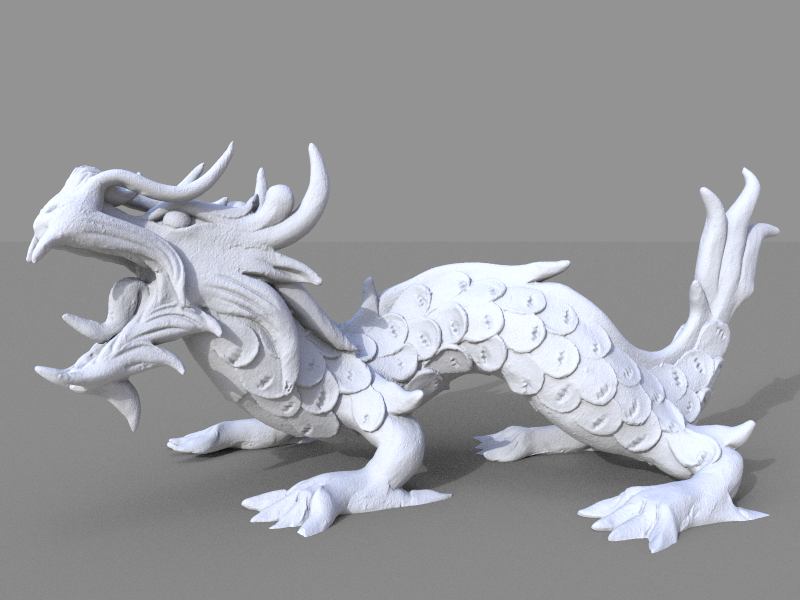
\includegraphics[width=\textwidth]{renders/xyzrgb_dragon_white}
        \caption{XYZRGB dragon. Scanned by Stanford Computer Graphics Laboratory}
    \end{subfigure}
    \begin{subfigure}{0.48\textwidth}
        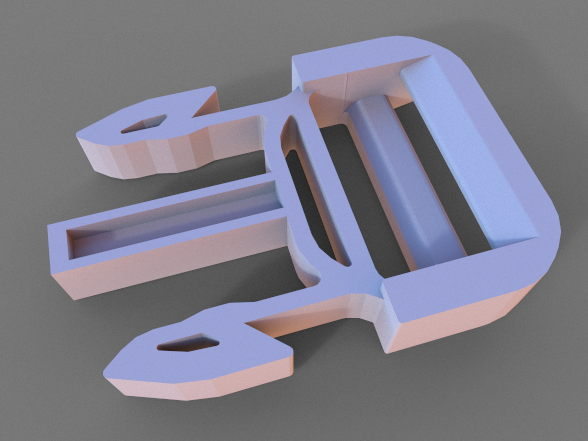
\includegraphics[width=\textwidth]{renders/buckle}
        \caption{Buckle. By Josip Vukovic from GrabCAD community digital library}
    \end{subfigure}
    \caption{3d models used for measurements}
    \label{fig:measurements_models}
\end{figure}

\subsection{Error measure}
\label{section:error_measure}
The \emph{Root Mean Square} (RMS) of the difference is a simple popular quantitative measure of the
error between two images. But it can not be used as a reasonable metric for comparison in our case,
because it depends too much on the absolute value of the image brightness difference. One example of
this is shown at figure \ref{fig:wrong_rms}. You can see the two pairs of images having similar RMS
error value $\approx 0.004$. But perceptual difference between two relatively dark images
\ref{fig:wrong_rms_dark} is considerably higher than one of brighter pair
\ref{fig:wrong_rms_bright}.
\begin{figure}[h]
    \centering
    \begin{subfigure}{0.4\textwidth}
        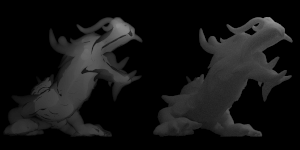
\includegraphics[width=\textwidth]{renders/matrix/rms000458}
        \caption{RMS=0.00458, high visual difference}
        \label{fig:wrong_rms_dark}
    \end{subfigure}
    \begin{subfigure}{0.4\textwidth}
        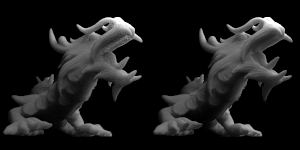
\includegraphics[width=\textwidth]{renders/matrix/rms000401}
        \caption{RMS=0.00401, low visual difference}
        \label{fig:wrong_rms_bright}
    \end{subfigure}
    \caption{Problem of RMS measure. Two pairs of images has close RMS error value. While perceived
    difference between the images of the left pair is much higher. Images are shown in 2x
    brightness}
    \label{fig:wrong_rms}
\end{figure}

That is why another metric was chosen. As a basis of calculation of the relative difference
between two images \emph{Normalized Cross-Correlation} was used:
\[
NCC = \frac{\sum_{x,y} (f(x,y)-\bar{f})(g(x,y)-\bar{g})}{N\sigma_f\sigma_g}
\]
where $f$ and $g$ are 2d functions $\bar{f}, \bar{g}$ are their mean values, $\sigma_f,\sigma_g$
respective standard deviations and $N$ is a number of pixels in case of images as a 2d functions.

General case of Cross-Correlation is often used for template matching in image processing. But in
our case it helps to measure the difference between two functions $f$ and $g$ regardless of their
mean value. Thus, it allows us to compute the error measure between various pairs of images
independent of their absolute average brightness. However, using only the \gls{NCC} for measuring
the error is not enough. For the purpose of better representation and visualization of the results,
we re-parametrized the NCC value in the following way:
\begin{equation}
\label{eq:cvalue}
C = \frac{\bar{f}}{\bar{g}}\frac{NCC^2-0.8}{0.2}
\end{equation}

This form helps to represent the images exposing the correlation with their reference only higher
than 0.8 within the range [0,1].
The reason for this is that pairs with the NCC value lower than 0.8 are appeared to be unacceptable
visually wrong and can be discarded.
The factor $\bar{f}/\bar{g}$ is the ratio between average image brightness. It accounts for
relative difference of the Diffusion approximation image with the reference, not the absolute
difference, like in RMS case.

While using this metric, the images which appear very similar to their reference are represented by
C-value \ref{eq:cvalue} close to 1. And relatively wrong rendered images are having zero or near
zero C-values. Take a look at figure \ref{fig:both_set} for some examples of good and bad
correlation.
The path traced reference images are shown on the left.
\begin{figure}[h]
    \centering
    \begin{subfigure}{0.48\textwidth}
        
\includegraphics[width=\textwidth]{{{renders/matrix/area_buckle_da_100.0000_ds_0.0500}}}
        \caption{Buckle, area light. $1/\sigma_a=1000mm, 1/\sigma_s=0.5mm, C=0.745$}
    \end{subfigure}
    \quad
    \begin{subfigure}{0.48\textwidth}
        
\includegraphics[width=\textwidth]{{{renders/matrix/env_buckle_da_0.2000_ds_0.1000}}}
        \caption{Buckle, IBL. $1/\sigma_a=2mm, 1/\sigma_s=1mm, C=0.009$}
    \end{subfigure}
    \newline
    \begin{subfigure}{0.48\textwidth}
        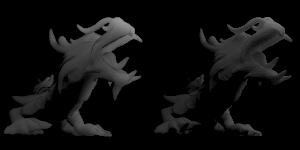
\includegraphics[width=\textwidth]{{{renders/matrix/area_dragon_da_1.0000_ds_0.2000}}}
        \caption{Dragon, area light. $1/\sigma_a=10mm, 1/\sigma_s=2mm, C=0.104$}
    \end{subfigure}
    \quad
    \begin{subfigure}{0.48\textwidth}
        
\includegraphics[width=\textwidth]{{{renders/matrix/env_dragon_da_30.0000_ds_0.0500}}}
        \caption{Dragon, IBL. $1/\sigma_a=300mm, 1/\sigma_s=5mm, C=0.793$}
    \end{subfigure}
    \caption{Two geometric shapes under two light setups. Left images of each pair is rendered using
    path tracing, right with Diffusion approximation. Examples of good and bad correlation using
    C-value metric \ref{eq:cvalue}}
    \label{fig:both_set}
\end{figure}

\subsection{Results of the simulations and discussion}
\label{section:measurements_results}
Here we present the generalized results of the measurements described in two previous sections.

To visualize the data we have chosen to plot the minimum correlation value for every given point out
of 4 different setups (2 models with 2 lighting conditions). In the other words, the worst output is
shown in the final heat map. This helps us to make more general conclusions. Even in the case when
Diffusion approximation is consistent enough with the reference in three of four cases, we still
choose the worst measure.

As seen on the figure \ref{fig:material_props}, the parameter space is roughly divided into two
regions. Samples with parameters from the dark red region have shown poor similarity with the Monte
Carlo references mostly due to high transparency of the objects with $\sigma_s<1 mm^{-1}$,
independent of the absorption coefficient of the material. Decreasing of the scattering even more
(i.e. increasing of the scattering distance $1/\sigma_s$) will lead to the pure glasses with no
noticeable scattering. This case would represent top and top right regions out of the graph limits.
These materials are not intended to be rendered with Diffusion approximation. The 

Materials with low scattering at the top left corner are not transparent due to the high absorption.
But the high error and low correlation in this case may be explained by the fact that the low albedo
materials are poorly approximated by Diffusion approximation in general. The order values of
$\alpha=\sigma_s/(\sigma_s+\sigma_a)$ in that region is about 0.1-1\%.

Lower part of the graph stands for highly scattering materials with mean free scattering path length
much smaller than the characteristic scale of the object's geometric details. This means the light
experience many scattering events before leaving the surface. As expected, these points display high
correlation. The effect of low albedo in the bottom lower corner does not exposed too much. The
lowest volumetric albedo value $\alpha=\sigma_s/(\sigma_s+\sigma_a)=0.9$  in that region. Materials
with their properties far left out of the plot would represent too dark objects regardless of the
rendering method.
The space far bottom out of the graph would stand for the objects with so much scattering
contribution (i.e. very short mean free path length), that it is impractical to render them with
BSSRDF model.
The classical BRDF approach will result in the same output avoiding complicated SSS computation.

\begin{figure}[h]
    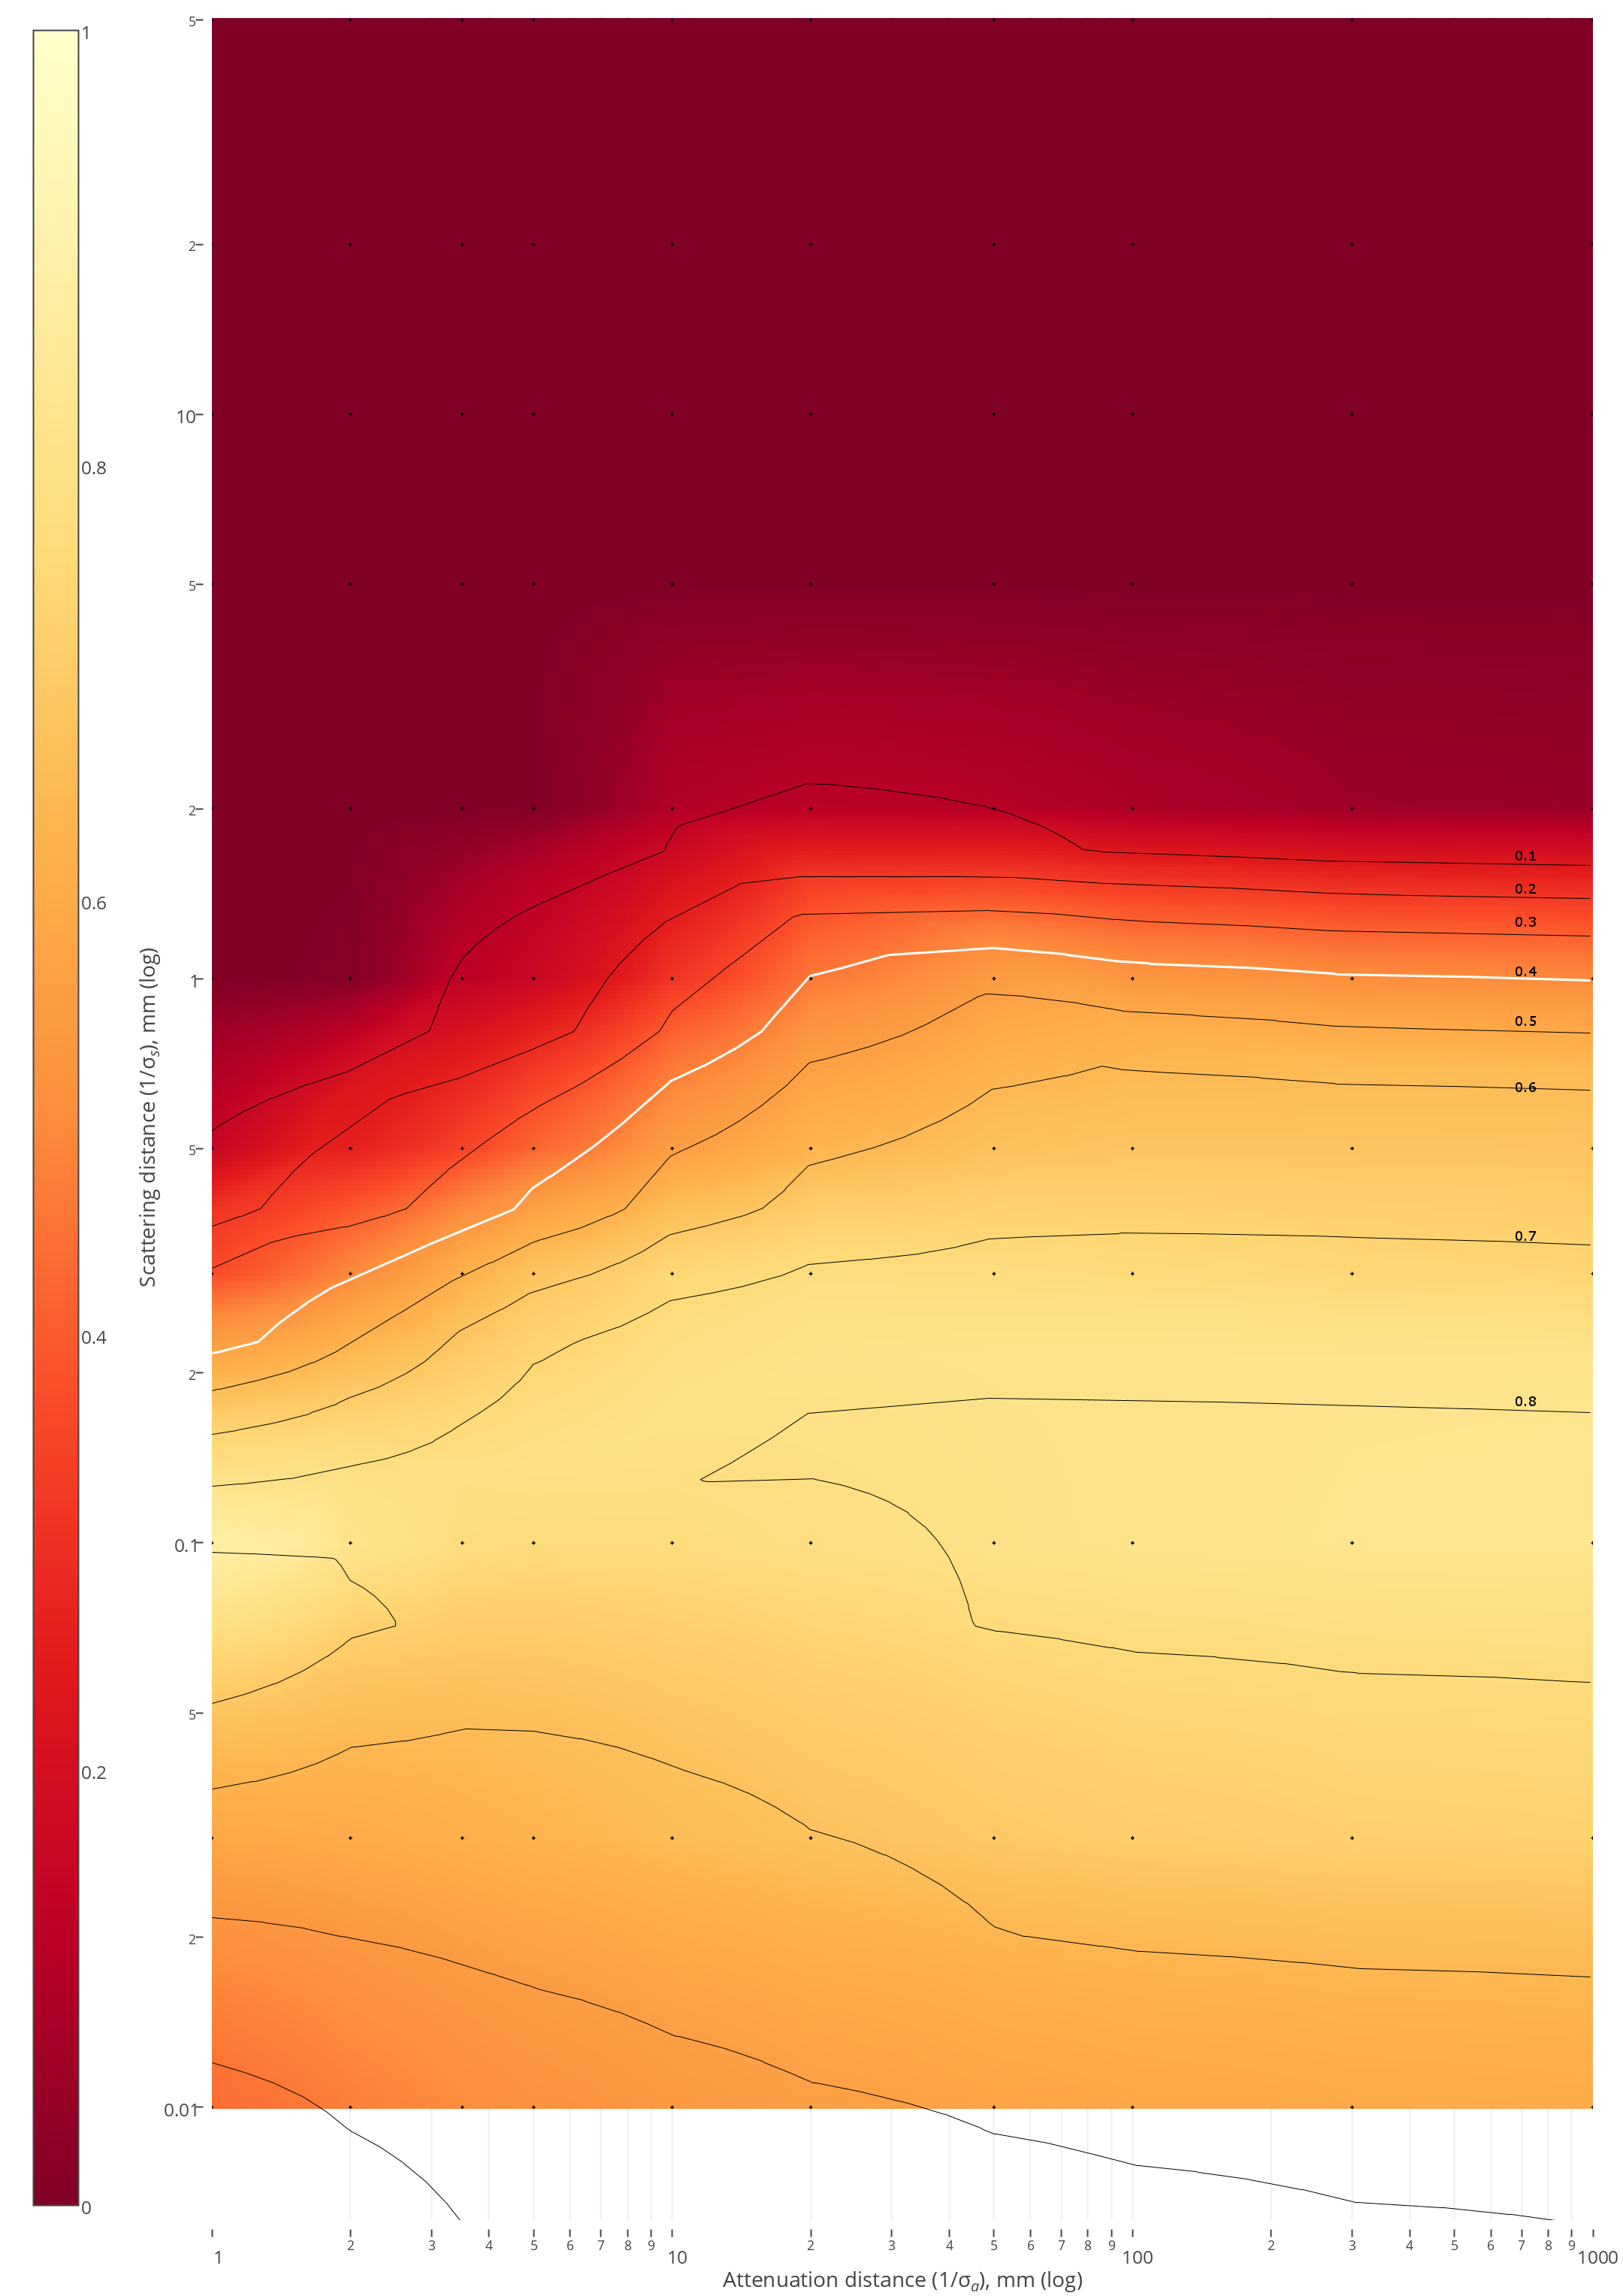
\includegraphics[width=\textwidth]{plots/matrix_isocontours} \caption{Aggregated heat map of the
    SSS properties analysis. Minimal C-value correlation of four experiments is color coded (see
    details at section \ref{section:error_measure}. Approximate isocontour on the level of 0.4 is
    considered as threshold. All the point with correlation higher than this level represents the
    relatively good match of the Diffusion approximation and the Monte Carlo reference}
    \label{fig:material_props}
\end{figure}

\subsubsection{Measured data sources}
The next step is to compare the measured optical properties of the real world materials and find out
how good they can be approximated.

There are a number of data sources with scattering coefficients available in the literature.
 
Scattering coefficients can be acquired by measuring diffusion profiles from a real-world object by
analyzing scattering of a laser beam \cite{Jensen:2001:PMS:383259.383319}.

Acquisition of the optical properties of human skin is a wide and important topic as
itself. Structured light patterns, for example, were used to estimate scattering coefficients of
different types of skin in \cite{tariq_efficient_2006-1}.

Rendering of translucent liquids is a bad potential case for rendering by Diffusion approximation
\textit{a priori}. Nevertheless the study of \cite{Narasimhan:2006:ASP:1141911.1141986}, containing
a big variety of liquids measured by dilution, appeared to be a valuable source of data.

The most recent up to date and comprehensive set of measured results is available in the work by
\cite{Gkioulekas:2013:IVR:2508363.2508377}. The advanced inverse volume rendering framework used in
that study allowed to take into account multiple scattering events and measure solids that are not
possible to dilute.

Selected data regions from all of these sources were used to estimate applicability of the Diffusion
approximation. The following table \ref{table:material_dataq} shows the minimum and maximum values
of mean free path absorption and scattering length out of different R,G or B channel. The plotted
regions at figure \ref{fig:material_props_data} represent the approximate location of the material
with respect of this bounds.
\begin{table}[h]
\begin{tabu} to 0.6\textwidth { |l |c|c|c|c| c| }
    \hline
    Material & min $1/\sigma_a$, mm & max $1/\sigma_a$, mm & min $1/\sigma_s$, mm & max
    $1/\sigma_s$, mm & C-value \\ \hline
    \hline
    human skin & 2 & 20 & 0.66 & 1 & 0.1-0.4 \\ \hline
    whole milk & 30 & 100 & 0.007 & 0.008 & $0.6^*$ \\ \hline
    milk soap & 66 & 333 & 0.10 & 0.13 & 0.8 \\ \hline
    glycerin soap & 500 & 1000 & 4.0 & 5.5 & 0-0.05 \\ \hline
    hand cream & 80 & 90 & 0.025 & 0.5 & 0.7-0.8 \\ \hline
    liquid clay & 200 & 250 & 0.015 & 0.03 & 0.7 \\ \hline
    coffee & 15 & 25 & 2.5 & 3.7 & 0.05 \\ \hline
    red wine & 1.2 & 1.4 & 18.9 & 91 & 0 \\ \hline
    mustard & 2.2 & 16 & 0.05 & 0.16 & 0.7-0.8 \\ \hline
    robitussin & 200 & 500 & 20 & 83 & 0 \\ \hline
\end{tabu}
\caption{Data for the selected materials from the following sources
\cite{Jensen:2001:PMS:383259.383319}, \cite{tariq_efficient_2006-1},
\cite{Narasimhan:2006:ASP:1141911.1141986},
\cite{Gkioulekas:2013:IVR:2508363.2508377}.\newline $^*$ C-value for the whole milk is extrapolated}
\label{table:material_data}
\end{table}

From the plotted data in the figure \ref{fig:material_props_data} couple of conclusions could be
made.

First, the experiment matches the obvious expectation that materials with high transparency
like glycerin soap, robitussin or diluted liquids like red wine and coffee are the bad candidates to
be rendered with Diffusion approximation.

The lowest error to be expected from light and optically dense materials like milk soap, hand cream
or mustard.

The expected correlation $C\approx0.6$ for the whole milk is quite low, considering the bright and
dense look of the substance. However, qualitatively similar results for the light simulation in milk
is also reported in the \cite{Donner:2009:EBM}. Author makes the conclusion that rather
complicated microscopic structure of the fat molecules in water makes it difficult to be simulated
by approximation.

The human skin is located on the border of the acceptability. Dark skin is discarded due to
the low volume and surface albedo. And even objects with the characteristics of the
bright human skin are expected to have serious differences with the brute force Monte Carlo
simulated results.

\begin{figure}
    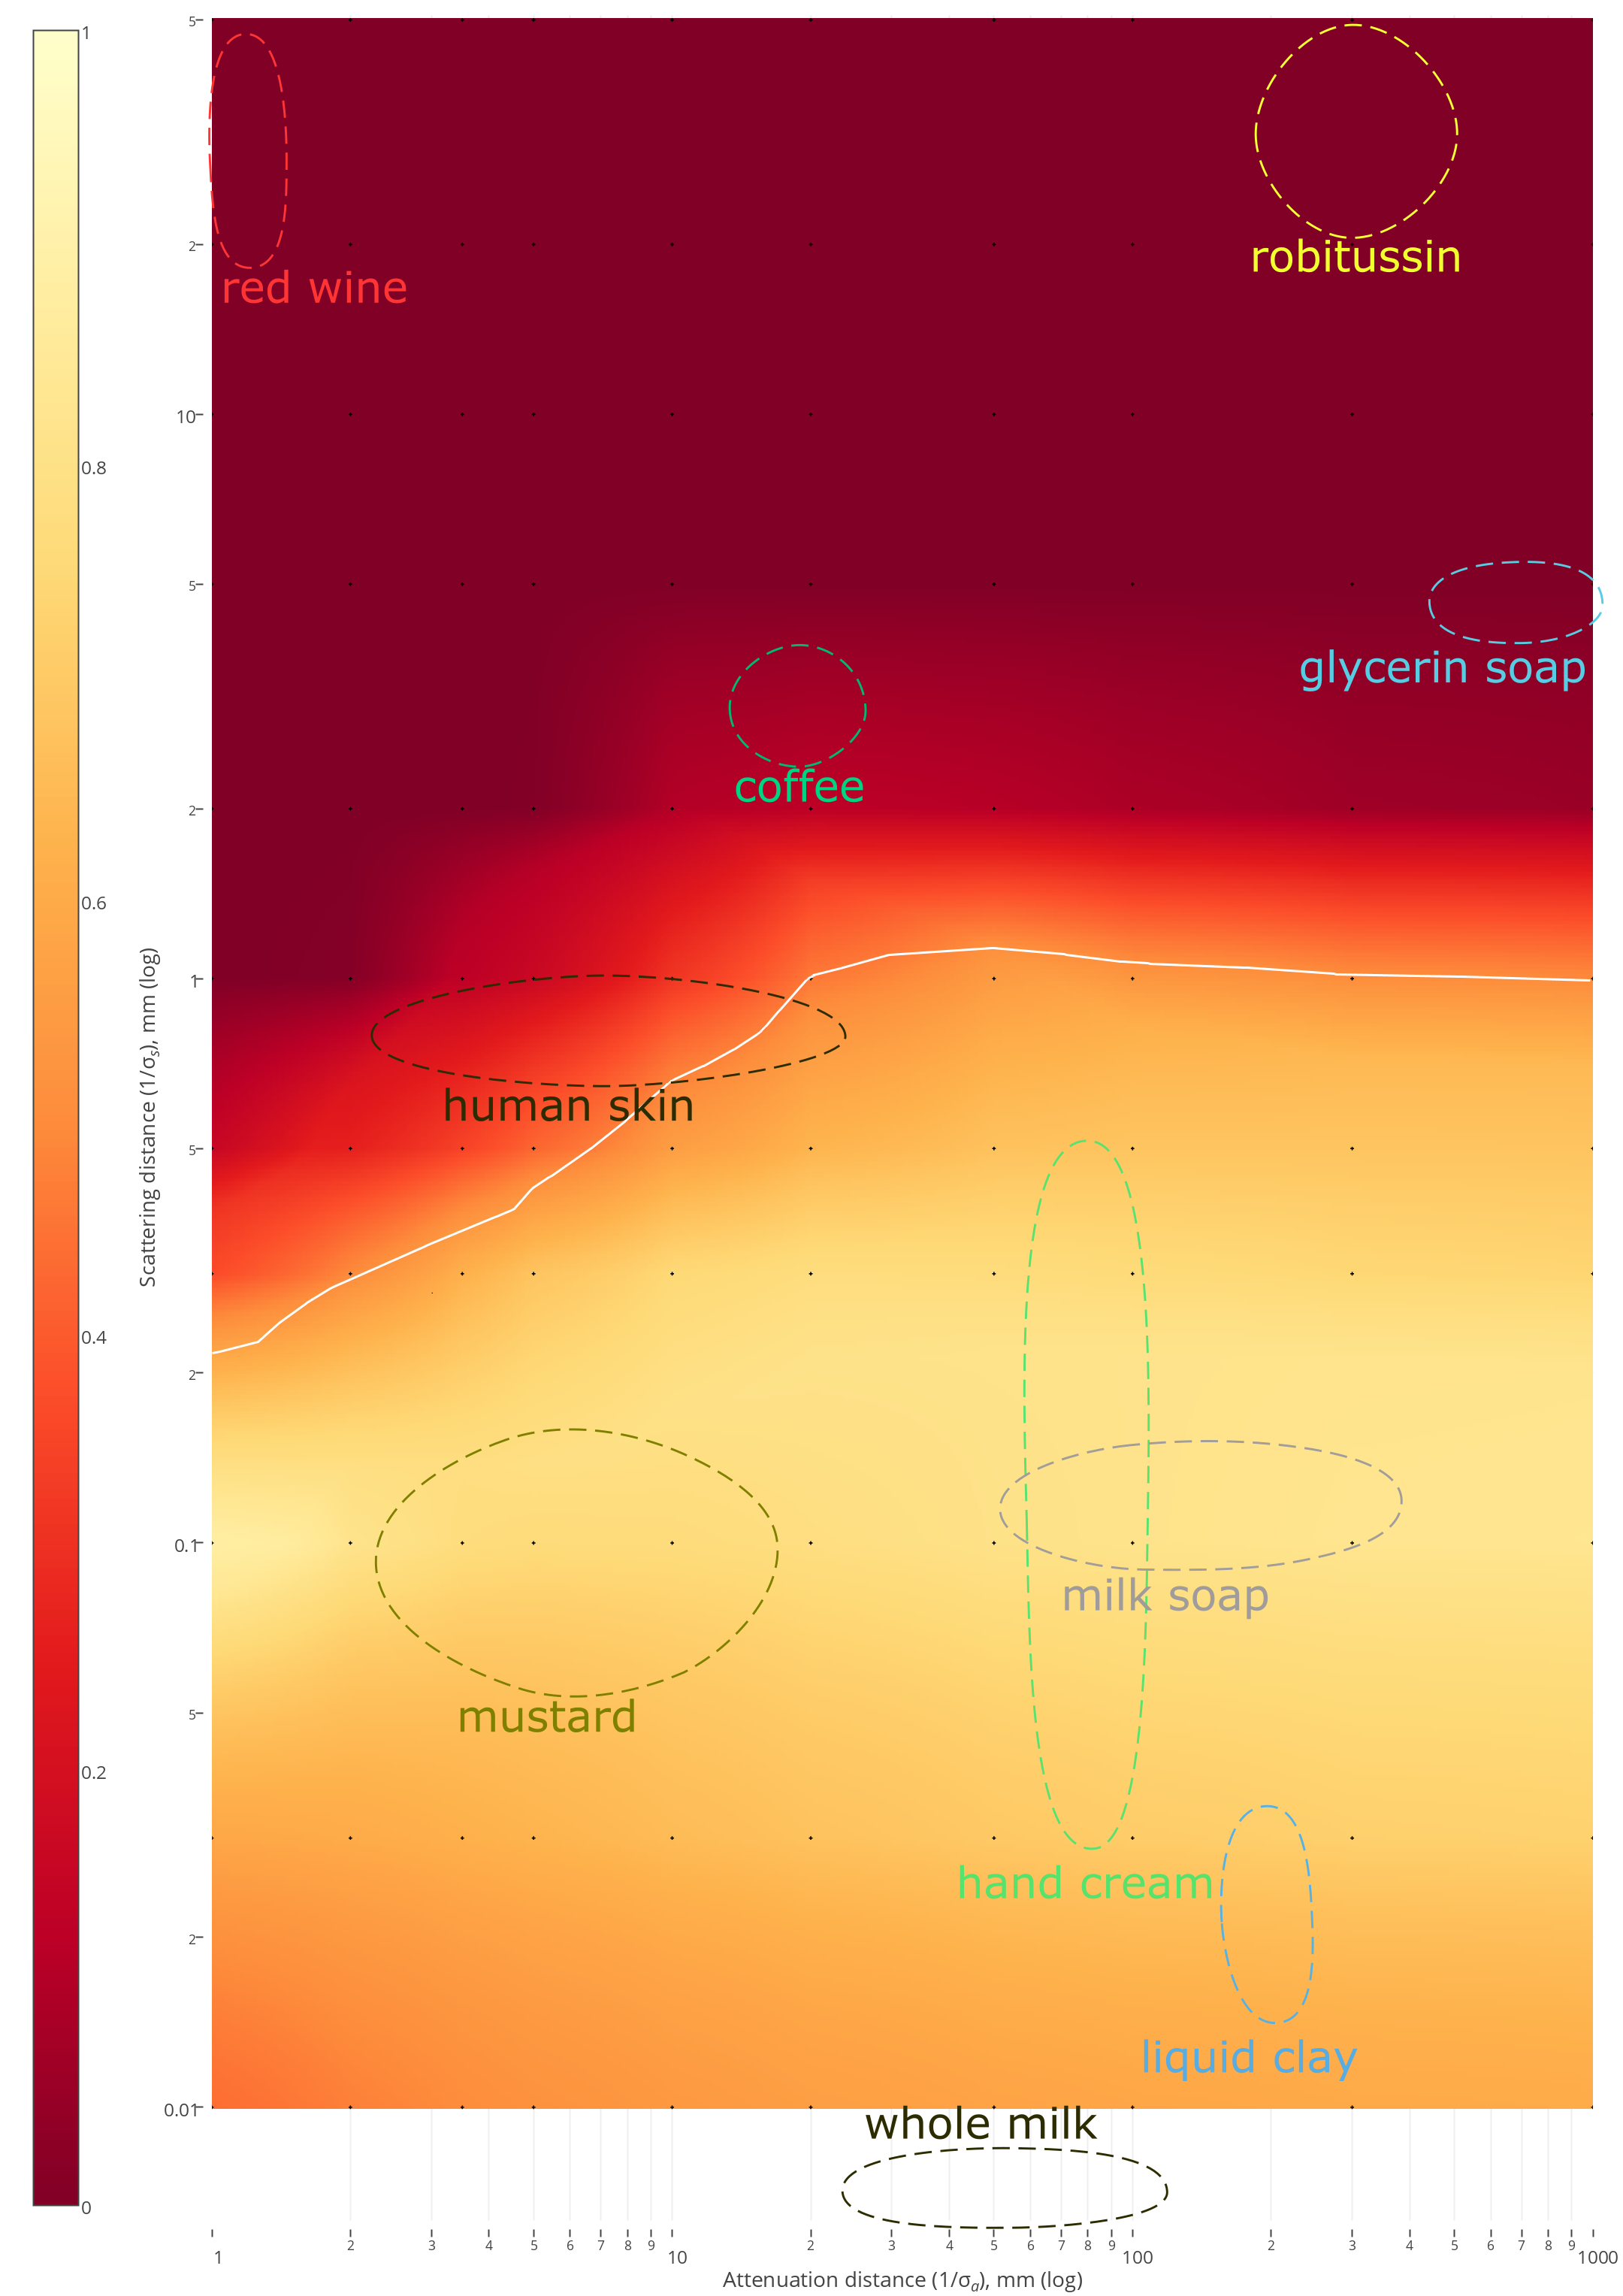
\includegraphics[width=\textwidth]{plots/matrix_data}
    \caption{Data from the table \ref{table:material_data} are approximately plotted over the
    correlation measure}
    \label{fig:material_props_data}
\end{figure}